\documentclass{article}
\usepackage{graphicx}
\usepackage{minted}
\usepackage{parskip}
\usepackage[colorlinks,
            urlcolor=blue]{hyperref}
%\usepackage[margin=1in]{geometry}
\usepackage{amsmath}
\usepackage{amssymb}
\usepackage{fancyvrb}
\usepackage{booktabs}
\usepackage{url}
\usepackage{hyperref}
\usepackage{multirow}
\usepackage{pbox}
\usepackage[margin=1in]{geometry}

\author{Ashwin Srinath}
\title{An OpenCL-based tridiagonal solver for evaluation
    of compact finite differences on Graphics Processing Units}
\begin{document}
% \renewcommand{\bibname}{References}

\section{Introduction}

The motivation for this work comes from the need to evaluate
\emph{compact finite differences} arising in large simulations of
combustion.

We consider the following fourth-order
compact finite difference scheme for evaluating the first derivative,
with a 3-point stencil:

\begin{equation}
    \alpha(f^{\prime}_{i-1} + f^{\prime}_{i+1}) + f^{\prime}_i
    =
    a\frac{f_{i+1} - f_{i-1}}{dx}
\end{equation}

For the particular scheme used, $\alpha = 1/4$,
and $ a = 3/4 $.
It is easily noted that this leads to a tridiagonal system of equations,
along with a 3-point stencil to evaluate the RHS.
Further, the left boundary can be treated using the following implicit equation:

\begin{equation}
    f^{\prime}_1 + 2f^{\prime}_2 = \frac{-5f_1 + 4f_2 + f_3}{dx}
\end{equation}

The right boundary ($f^{\prime}_{n-1}$) is treated by utilizing
the negative complex-conjugate of the Fourier image of the stencil
at $f^{\prime}_1$:

\begin{equation}
    f^{\prime}_{n-1} + 2f^{\prime}_{n-2}
    =
    \frac{5f_{n-1} - 4f_{n-2} - f_{n-3}}{dx}
\end{equation}

The tridiagonal system that needs to be solved for the derivatives,
then has an LHS of the form:

\[ %\arraycolsep=4pt
 \begin{bmatrix}
     1&2\\
     1/4&1&1/4\\
     &1/4&1&1/4\\
     &&1/4&1&1/4\\
     &&&1/4&1&1/4\\
     &&&&&\ddots\\
     &&&&&&\ddots\\
     &&&&&&&\ddots\\
     &&&&&&&2&1
  \end{bmatrix}
\]

And an RHS of the form:

\[
 \begin{bmatrix}
     -5f_1 + 4f_2 + f_3\\
     f_{3} - f_{1}\\
     f_{4} - f_{2}\\
     \vdots\\
     \vdots\\
     \vdots\\
     \vdots\\
     f_{n} - f_{n-2}\\
     5f_{n} - 4f_{n-1} - f_{3}
  \end{bmatrix}
\]

\section{Domain decomposition}

The compact finite differences need to be evaluated
at each grid point in the problem domain,
shown in \ref{fig:domain}.
Each grid point is represented as a cell in this representation.

The domain has been shown as partitioned into blocks \ref{fig:one-block}.
The blocks are three dimensional to facilitate
the computation of derivatives in all three coordinate directions
without incurring excessive communication costs.

While evaluating the derivative, each block is assigned to a ``compute unit'',
which may be a single core, a multi-core processor, or a GPU.
Each block may be thought of as a collection of ``lines'' of grid points
\ref{fig:one-line}.





% left, lower, right, upper
\begin{figure}[h]
\begin{center}
\includegraphics[trim={{100pt} {150pt} {100pt} {150pt}}, clip, height=250pt]{img/domain.eps}
\end{center}
\caption{Domain}
\label{fig:domain}
\end{figure}

\begin{figure}[ht]
\begin{minipage}[b]{0.45\linewidth}
\centering
\includegraphics[trim={{50pt} {150pt} {50pt} {150pt}}, clip, height=200pt]{img/one-block.eps}
\caption{Single block}
\label{fig:one-block}
\end{minipage}
\hspace{0.5cm}
\begin{minipage}[b]{0.45\linewidth}
\centering
\includegraphics[trim={{50pt} {150pt} {50pt} {150pt}}, clip, height=200pt]{img/one-thread.eps}
\caption{Single thread}
\label{fig:one-line}
\end{minipage}
\end{figure}




\begin{figure}[h]
\begin{center}
\includegraphics[trim={{100pt} {150pt} {100pt} {150pt}}, clip, height=300pt]{img/parallel-x.eps}
\end{center}
\caption{Parallel x}
\label{fig:parallel-x}
\end{figure}




\begin{figure}[h]
\begin{center}
\includegraphics[trim={{100pt} {150pt} {100pt} {150pt}}, clip, height=300pt]{img/parallel-yz.eps}
\end{center}
\caption{Parallel yz}
\label{fig:parallel-yz}
\end{figure}




\begin{figure}[h]
\begin{center}
\includegraphics[trim={{100pt} {150pt} {100pt} {150pt}}, clip, height=300pt]{img/parallel-both.eps}
\end{center}
\caption{Parallel-both}
\label{fig:parallel-both}
\end{figure}




\section{Parallelism}


\section{}


\end{document}
